
%% RSET Project / Seminar LaTex Template Version 1.0 - November 2023

\documentclass[12pt,a4paper,titlepage]{report}

% Page layout
\usepackage[left=2.8cm, right=2.2cm, top=3cm, bottom=2.5cm]{geometry}

% Graphics and figure handling
\usepackage{graphicx}        % for including graphics
\usepackage{float}           % for precise placement of figures and tables
\usepackage{caption}         % for caption adjustments
\usepackage{subcaption}      % for subfigures
\usepackage{tcolorbox}       % for colored boxes
% Mathematical symbols and environments
\usepackage{amsmath}         % for math symbols and environments
\usepackage{amssymb}         % for additional math symbols

% Fonts and symbols
\usepackage{latexsym}        % LASY symbols
\usepackage{eufrak}          % for Fraktur fonts
\usepackage{type1cm}         % scalable fonts

% Other useful packages
\usepackage{longtable}       % for tables that span multiple pages
\usepackage{listings}        % for code listings
\usepackage{xcolor}          % for color support in listings
\usepackage{pdfpages}        % for including PDF pages
\usepackage{url}             % for handling URLs
\usepackage{acro}            % for acronyms
\usepackage{titlesec}        % for section title formatting

% Formatting
\captionsetup{justification=centering}  % Centering captions

% Color and formatting for listings (code)
\lstset{basicstyle=\ttfamily, columns=fullflexible, frame=single, breaklines=true, postbreak=\mbox{\textcolor{red}{$\hookrightarrow$}\space}}

% Example new sectioning titles format (optional)
\titleformat{\section}{\normalfont\Large\bfseries}{\thesection}{1em}{}

% Additional packages if needed
\usepackage{epsfig}          % legacy support for PostScript figures


\definecolor{customgreen}{rgb}{0,0.6,0}
\definecolor{customgray}{rgb}{0.5,0.5,0.5}
\definecolor{custommauve}{rgb}{0.6,0,0.8}
\lstdefinelanguage{HTML}{
	sensitive=true,
	keywords={},
	otherkeywords={<, >, /},
	morecomment=[s]{<!--}{-->},
	morestring=[b]"
}


\lstset{ 
	basicstyle=\small,        % the size of the fonts that are used for the code
	breaklines=true,                 % sets automatic line breaking
	commentstyle=\color{customgreen},    % comment style
	firstnumber=1,                % start line enumeration with line 1000
	frame=single,	                   % adds a frame around the code
	keepspaces=true,                 % keeps spaces in text, useful for keeping indentation of code (possibly needs columns=flexible)
	keywordstyle=\color{blue},       % keyword style
	numbers=left,                    % where to put the line-numbers; possible values are (none, left, right)
	numbersep=10pt,                   % how far the line-numbers are from the code
	numberstyle=\tiny\color{customgray}, % the style that is used for the line-numbers
	rulecolor=\color{black},         % if not set, the frame-color may be changed on line-breaks within not-black text (e.g. comments (green here))
	showspaces=false,                % show spaces everywhere adding particular underscores; it overrides 'showstringspaces'
	showstringspaces=false,          % underline spaces within strings only
	showtabs=false,                  % show tabs within strings adding particular underscores
	stepnumber=1,                    % the step between two line-numbers. If it's 1, each line will be numbered
	stringstyle=\color{custommauve},     % string literal style
	tabsize=2,	                   % sets default tabsize to 2 spaces
	title=\lstname                   % show the filename of files included with \lstinputlisting; also try caption instead of title
}


\titleformat{\chapter}[display]
{\normalfont\Large\bfseries\centering}{\chaptertitlename\
	\thechapter}{25pt}{\Large}
\titleformat{\section}{\normalfont\bfseries}{\noindent\thesection}{20pt}{}
\titleformat{\subsection}{\normalfont\small\bfseries}{\thesubsection}{15pt}{\small}
\titlespacing*{\chapter}{0pt}{0pt}{40pt}


\begin{document}
\titlepage
\thispagestyle{empty}
\begin{center}
	
\includegraphics[scale=0.35]{Figures/logo1.png}\\[0.2cm]
	\large \textit{Project Phase II Report On}\\[0.3cm]
	\Large \textbf{Advanced Supply and Trade Resource Optimisation (A.S.T.R.O.)}\\[0.3cm]
	\textit{Submitted in partial fulfillment of the
		requirements for the award of the degree of}\\[0.3cm]
	{\huge {$\mathfrak {Bachelor\; of\; Technology}$}}\\[.3cm]
	%{\Large {$\mathfrak {In}$}}\\[.5cm]
	%{\Large {$\mathfrak {Computer\; Science\; \&\; Engineering}$}}\\[2cm]
	\textit{in}\\[.2cm]
	{\Large \bf \itshape{{Computer Science and Business Systems}}}\\[0.7cm]
	\large \bfseries{By}\\[.1cm]
	\large \bfseries{Amel Chandra (U2109009)}\\[0.2cm]
	\large \bfseries{Bharath S. (U2109018)}\\[0.2cm]
	\large \bfseries{Joepaul Vilsan (U2109033)}\\[0.2cm]
	\large \bfseries{Shane George Salphie (U2109063)}\\[0.2cm]
	\large \bfseries{Under the guidance of}\\[0.3cm]
	\large \bfseries{Dr. Nikhila T. Bhuvan}\\[0.2cm]
	%		\includegraphics[width=8.0cm]{logo (1).jpg}\\[0.5cm]
	\large \textbf{Department of Computer Science and Business Systems}\\
	\large \textbf{Rajagiri School of Engineering \&\ Technology (Autonomous)}\\
	\small \bfseries{(Parent University: APJ Abdul Kalam Technological University)}\\
	\large \textbf{Rajagiri Valley, Kakkanad, Kochi, 682039}\\[0.2cm]
	\large \bfseries{April 2025}
\end{center}

\newpage
\thispagestyle{empty}
\vspace{1cm}
\begin{center}
	%	\textbf {DEPARTMENT OF COMPUTER SCIENCE \&\ ENGINEERING}\\
	%	\small \textbf{RAJAGIRI SCHOOL OF ENGINEERING \&\ TECHNOLOGY (AUTONOMOUS)}\\

	%	\small \textbf{RAJAGIRI VALLEY, KAKKANAD, KOCHI, 682039}\\
	%   \small \bfseries{(Affiliated to APJ Abdul Kalam Technological University)}\\[0.5cm]
	%\begin{figure}[htbp]
	%	\centering
	%\includegraphics[scale=0.40]{logo (1).jpg}
	%   \includegraphics[width=8.0cm]{logo (1).jpg}\\[0.5cm]
	%\end{figure}
	\large \bfseries{\huge{CERTIFICATE}}\\[1cm]
\end{center}

\renewcommand{\baselinestretch}{1.2}\normalsize

\sloppy
\emph{This is to certify that the project report entitled \textbf{”Advanced Supply and Trade Resource Optimisation”} is a bonafide record of the work done by \textbf{\mbox{Amel Chandra} (U2109009), \mbox{Bharath S (U2109018)}, \mbox{Joepaul Vilsan (U2109033)}, \mbox{Shane} \mbox{George} \mbox{Salphie (U2109063)}}, submitted to the Rajagiri School of Engineering \& Technology (RSET) (Autonomous) in partial fulfillment of the requirements for the award of the degree of Bachelor of Technology (B. Tech.) in "Computer Science and Business Systems" during the academic year 2024-2025.}\\[2.5cm]

\begin{flushleft}


	\begin{longtable}{p{5.8cm} p{5.8cm} p{5.8cm}}
		{Dr. Nikhila T. Bhuvan} & {Mr. Mahesh K.M.}      & {Dr. Divya James}     \\
		{Project Guide}         & {Project Co-ordinator} & {Head Of Department}  \\
		{Associate Professor}   & {Assistant Professor}  & {Associate Professor} \\
		{Dept. of CU}           & {Dept. of CU}          & {Dept. of CU}         \\
		{RSET}                  & {RSET}                 & {RSET}                \\
	\end{longtable}
\end{flushleft}
\vspace{2cm}






\renewcommand{\baselinestretch}{1.5}\normalsize
\newpage
%\renewcommand\abstractname{ACKNOWLEDGEMENTS}
\chapter*{ACKNOWLEDGMENT}
%\begin{abstract}
\pagenumbering{roman}
\setcounter{page}{1}
\addcontentsline{toc}{chapter}{Acknowledgment}
\vspace{1.5cm}
%\begin{spacing}{}
\paragraph\ We wish to express my sincere gratitude towards \textbf{Rev. Dr. Jaison Paul Mulerikkal}, Principal of RSET, and \textbf{Dr. Divya James}, Head of the Department of Computer Science and Business Systems for providing us with the opportunity to undertake my project, \textbf{"Advanced Supply and Trade Resource Optimisation"}.
\paragraph\ We are highly indebted to our project coordinators, \textbf{Dr. Nikhila T Bhuvan}, Associate Professor, Department of Computer Science and Business Systems, \textbf{Ms. Ancy C A}, Assistant Professor, Department of Computer Science and Business Systems,\textbf{Mr. Mahesh K M} Assistant Professor,Department of Computer Science and Business Systems for their valuable support.

\paragraph\ It is indeed my pleasure and a moment of satisfaction for me to express my sincere
gratitude to my project guide \textbf{Dr. Nikhila T Bhuvan} for her patience and all the priceless advice and wisdom she has shared with me.
\paragraph\ Last but not the least, I would like to express my sincere gratitude towards all other teachers and friends for their continuous support and constructive ideas.
%\end{spacing}
\begin{flushright}
	\textbf{Amel Chandra}\\
	\textbf{Bharath S}\\
	\textbf{Joepaul Vilsan}\\
	\textbf{Shane George Salphie}
\end{flushright}


\newpage

\renewcommand{\baselinestretch}{1.5}\normalsize

\chapter*{Abstract}
\addcontentsline{toc}{chapter}{Abstract}
\vspace{1.5cm}
\paragraph{}\ \ \ \ Small-scale vendors face significant challenges in competing with large retail chains due to limited purchasing power, inefficient logistics, and restricted access to financial services. These barriers often hinder their ability to manage demand fluctuations and make informed business decisions, threatening their long-term sustainability. This project aims to address these issues by developing a comprehensive platform that empowers small vendors through collaborative purchasing, optimized logistics, and data-driven decision-making. By enabling vendors to combine orders, the platform facilitates bulk purchasing, unlocking competitive discounts and cost savings. Advanced algorithms optimize logistics by streamlining delivery routes, thereby reducing transportation costs and enhancing operational efficiency.  These features empower vendors to make strategic decisions that align with market demands and their business goals. The ultimate goal is to level the playing field for small vendors, enabling them to compete effectively with larger retail chains while fostering sustainable growth in local economies. The deliverables of this project include a fully functional platform supporting vendor collaboration and an optimized logistics module to reduce operational costs. By promoting economic resilience, enhancing competitiveness, and driving sustainable development, this project seeks to strengthen the local vendor ecosystem and contribute to the overall development of communities.

%\end{spacing}
%\end{abstract}


\newpage
\normalsize{}

%\pagenumbering{roman}
%\setcounter{page}{4}
%\begin{spacing}{}
\tableofcontents
%\end{spacing}
% \thispagestyle{empty}
\newpage

\chapter*{List of Abbreviations}
\addcontentsline{toc}{chapter}{List of Abbreviations}

ASTRO - Advanced Supply and Trade Resource Optimisation \\
SDG - Sustainable Development Goals \\
API - Application Programming Interface \\
ACO - Ant Colony Optimisation \\
GA - Genetic Algorithm \\
SME - Small to Medium-sized Enterprises \\
UI - User Interface \\
MOQ - Minimum Order Quantity \\
EAGA - Environment Adaptive Genetic Algorithm \\
EAACO - Environment Adaptive Ant Colony Optimisation \\
DBSCAN - Density-Based Spatial Clustering of Applications with Noise \\
KNN - K-Nearest Neighbours \\

\newpage

\listoffigures
\addcontentsline{toc}{chapter}{List of Figures}
% \thispagestyle{empty}
\newpage


% \pagenumbering{roman}
%\setcounter{page}{9}
\listoftables
\addcontentsline{toc}{chapter}{List of Tables}
%	\addcontentsline{toc}{chapter}{List of Abbreviations}
%	\listof{Abbreviations}
% \thispagestyle{empty}
\newpage



\cleardoublepage

\pagenumbering{arabic}
\setcounter{page}{1}

\chapter{Introduction}

Small-scale vendors are essential contributors to local economies, offering unique products and
personalized services that enrich communities. However, they face significant challenges
competing against large retail chains, which benefit from greater purchasing power, efficient
logistics, and easier access to financial resources. Due to limited resources, small vendors often
struggle with high supply costs, fragmented logistics, and restricted access to credit, hindering
their ability to grow and compete effectively.
The ASTRO (Advanced Supply and Trade Resource Optimization) platform addresses these
challenges by providing a comprehensive solution that empowers small vendors through
collaborative purchasing, logistics optimization, and data-driven financial services. By allowing
vendors to pool orders, ASTRO enables them to achieve bulk pricing similar to large retailers,
reducing per-unit costs and enhancing profitability. The platform also incorporates advanced
logistics optimization algorithms, improving delivery efficiency and reducing operational
expenses. Additionally, ASTRO offers financial services based on transaction data, enabling
vendors to access credit and make informed decisions for business expansion.

ASTRO’s functionality extends further with real-time demand forecasting tools, equipping
vendors with predictive insights that help manage inventory and adapt to changing market
demands. Through these features, ASTRO not only improves individual vendor competitiveness
but also fosters economic resilience in local communities by supporting sustainable growth and
operational efficiency. As a result, ASTRO is positioned as a vital resource for small vendors,
helping them navigate a competitive retail landscape while contributing to the stability and
diversity of local economies.
\section{Background}

Small-scale vendors are integral to the fabric of local economies, providing unique products,
personalized services, and fostering vibrant community interactions that larger retail chains
often cannot replicate. These vendors contribute significantly to economic diversity, cultural
richness, and employment within their communities. However, despite their crucial role,
small-scale vendors face persistent challenges that impede their ability to compete effectively
with larger retail entities. These challenges include limited purchasing power, inefficient logistics,
restricted access to financial services, and a lack of data-driven decision-making tools.
In today’s highly competitive retail landscape, large retail chains leverage economies of scale to
negotiate bulk purchasing discounts, implement sophisticated logistics networks, and utilize
advanced data analytics to optimize their operations and marketing strategies. In contrast,
small-scale vendors typically operate with constrained resources, making it difficult for them to
achieve similar efficiencies and cost-effectiveness. This disparity not only affects their
profitability but also limits their capacity to respond to market fluctuations and evolving
consumer demands.
The ASTRO platform (Advanced Supply and Trade Resource Optimization) is designed to
address these disparities by providing small-scale vendors with tools and services that enhance
their competitive edge. By enabling collaborative purchasing, optimizing logistics, and offering
data-driven financial services, ASTRO empowers local vendors to achieve bulk pricing,
streamline their operations, and make informed business decisions. This platform aims to bridge
the gap between small vendors and large retail chains, fostering economic resilience and
sustainable growth within local communities.
Moreover, the advent of digital transformation has revolutionized various industries, including
retail. The integration of technology into traditional business models is essential for small-scale
vendors to remain relevant and competitive. ASTRO leverages modern technological
advancements, such as machine learning algorithms for logistics optimization and predictive
analytics for demand forecasting, to deliver practical solutions tailored to the specific needs of
small vendors. The significance of ASTRO extends beyond individual business success; it
contributes to the overall economic health of communities by supporting the sustainability and
growth of small-scale enterprises.

\section{Problem Definition}

Small-scale vendors face a significant challenge in today’s competitive retail landscape, where large retail chains dominate with bulk pricing, advanced logistics, and extensive resources. This disparity puts small vendors at a disadvantage, as they often lack the economies of scale and infrastructure necessary to compete effectively. The problem is that, despite being crucial to local economies, small vendors struggle with high operational costs, inefficient logistics, and limited access to affordable credit, all of which hinder their ability to grow sustainably. This issue is exacerbated by the lack of platforms that cater to the specific needs of small-scale businesses, especially when it comes to aggregating demand, optimizing supply chains, and improving cash flow.

Without access to bulk purchasing and efficient logistics, small vendors pay higher prices for goods, limiting their profit margins and making it difficult to reinvest in their businesses. Furthermore, the absence of accurate demand forecasting and inventory management tools leads to overstocking or stockouts, reducing customer satisfaction and revenue. These issues underscore the need for a system that enables small vendors to pool their purchasing power, streamline their supply chains, and make data-driven decisions to improve their competitiveness.

The Advanced Supply and Trade Resource Optimization (A.S.T.R.O.) platform seeks to address this gap by providing small-scale vendors with the tools to compete with larger retail chains. A.S.T.R.O. enables collaborative purchasing, allowing vendors to aggregate their orders and access bulk discounts, thus reducing product costs. Additionally, the platform offers real-time demand forecasting, helping vendors optimize inventory levels to avoid both overstock and stockouts. To address financial limitations, A.S.T.R.O. includes data-driven financial services, such as credit assessment and tailored loans, designed to enhance cash flow and support business growth.

By facilitating these services, A.S.T.R.O. aims to foster economic resilience and sustainable growth in local communities. Its focus on empowering small vendors with advanced tools levels the playing field, promoting a more equitable and competitive market environment. This approach not only ensures that small vendors can thrive but also contributes to the overall health and diversity of the retail ecosystem.

\section{Scope and Motivation}
The ASTRO platform is a multifaceted solution designed to support small-scale vendors by addressing key operational challenges through technological integration and collaborative strategies. The scope of ASTRO encompasses the development and implementation of several core functionalities:

\begin{enumerate}
	\item \textbf{Collaborative Purchasing:} ASTRO facilitates group purchasing among small vendors, allowing them to pool their orders to achieve bulk pricing discounts. This feature enhances purchasing power, enabling vendors to reduce their cost of goods sold and improve profit margins.

	\item \textbf{Logistics Optimization:} Utilizing advanced algorithms, ASTRO optimizes delivery routes to reduce transportation costs and improve delivery efficiency. By streamlining logistics, the platform helps vendors achieve timely deliveries and minimize operational expenses.

	\item \textbf{Real-Time Demand Forecasting:} Leveraging predictive analytics, ASTRO provides real-time demand forecasting tools that help vendors anticipate market demand and manage inventory levels effectively. Accurate demand forecasting reduces the risk of overstocking or stockouts, ensuring that vendors can meet customer needs efficiently.

	\item \textbf{User-Friendly Interface:} ASTRO is designed with an intuitive user interface that ensures ease of use for vendors with varying levels of technical expertise. This feature maximizes user engagement and ensures that vendors can effectively utilize the platform’s functionalities to enhance their business operations.
\end{enumerate}

The motivation behind ASTRO stems from the urgent need to empower small-scale vendors in an increasingly competitive retail environment. As large retail chains continue to dominate the market through superior purchasing power and advanced logistics, small vendors risk marginalization and potential business failure. ASTRO addresses these challenges by providing a robust platform that enhances operational efficiency, reduces costs, and increases access to financial resources, thereby enabling small vendors to compete on a more equal footing.

Additionally, ASTRO is motivated by the broader goal of fostering economic resilience and sustainability within local communities. Small-scale vendors are pivotal to the economic diversity and vitality of local markets, contributing to job creation and community development. By supporting these vendors, ASTRO not only enhances individual business success but also strengthens the overall economic fabric of communities, promoting long-term sustainable growth and economic stability.
\section{Objectives}
The ASTRO project is guided by a set of clear and actionable objectives aimed at addressing the challenges faced by small-scale vendors. These objectives are designed to enhance operational efficiency, reduce costs, and provide financial support, thereby empowering vendors to compete effectively in the marketplace. The primary objectives of ASTRO include:

\begin{enumerate}
	\item \textbf{Enable Collaborative Purchasing:}
	      \begin{itemize}
		      \item \textbf{Objective:} Develop a robust system that allows small vendors to combine their orders, thereby achieving bulk purchasing discounts.
		      \item \textbf{Outcome:} Increased purchasing power, reduced cost of goods sold, and improved profit margins for vendors.
	      \end{itemize}

	\item \textbf{Optimize Logistics:}
	      \begin{itemize}
		      \item \textbf{Objective:} Implement advanced route optimization algorithms to streamline delivery processes, reduce transportation costs, and enhance operational efficiency.
		      \item \textbf{Outcome:} Cost-effective logistics operations, timely deliveries, and reduced operational expenses.
	      \end{itemize}

	\item \textbf{Provide Real-Time Demand Forecasting:}
	      \begin{itemize}
		      \item \textbf{Objective:} Integrate predictive analytics tools to offer real-time demand forecasting, enabling vendors to anticipate market demand and manage inventory levels effectively.
		      \item \textbf{Outcome:} Minimization of overstocking and stockouts, improved inventory management, and enhanced ability to meet customer demands.
	      \end{itemize}


	\item \textbf{Promote Economic Resilience and Sustainability:}
	      \begin{itemize}
		      \item \textbf{Objective:} Foster economic resilience by providing small vendors with the tools and resources needed to sustain and grow their businesses.
		      \item \textbf{Outcome:} Long-term sustainability, increased competitiveness, and strengthened economic stability within local communities.
	      \end{itemize}

	\item \textbf{Enhance User Experience and Accessibility:}
	      \begin{itemize}
		      \item \textbf{Objective:} Design a user-friendly interface that ensures easy access to the platform’s features, regardless of vendors’ technical expertise.
		      \item \textbf{Outcome:} High user engagement, effective utilization of platform functionalities, and improved overall user satisfaction.
	      \end{itemize}

	\item \textbf{Support Community Development:}
	      \begin{itemize}
		      \item \textbf{Objective:} Encourage collaboration and mutual support among vendors, fostering a sense of community and shared growth.
		      \item \textbf{Outcome:} Collective bargaining power, knowledge sharing, and resource optimization, leading to a stronger and more cohesive vendor network.
	      \end{itemize}
\end{enumerate}

By achieving these objectives, ASTRO aims to create a comprehensive solution that empowers small-scale vendors to overcome their operational challenges, enhance their competitiveness, and contribute to the sustainable growth of local economies. Each objective is strategically aligned to address specific pain points, ensuring that the platform delivers tangible benefits and drives meaningful improvements in vendors' business operations.




\section{Relevance}

The relevance of the ASTRO project is multifaceted, addressing critical needs within the retail ecosystem and contributing to broader economic and social goals. Key aspects of ASTRO’s relevance include:

\begin{enumerate}
	\item \textbf{Economic Empowerment of Small Vendors:}
	      \begin{itemize}
		      \item \textbf{Impact:} ASTRO directly addresses the economic challenges faced by small-scale vendors, enhancing their purchasing power and optimizing logistics cost. This empowerment enables vendors to operate more efficiently, reduce costs, and increase profitability, thereby improving their economic standing and sustainability.
	      \end{itemize}

	\item \textbf{Enhancing Local Economies:}
	      \begin{itemize}
		      \item \textbf{Impact:} By supporting small vendors, ASTRO contributes to the vitality and resilience of local economies. Small businesses are integral to economic diversification and job creation, promoting the long-term sustainability of local markets.
	      \end{itemize}

	\item \textbf{Technological Advancement and Digital Transformation:}
	      \begin{itemize}
		      \item \textbf{Impact:} ASTRO exemplifies the role of technology in transforming traditional business models. By leveraging advanced algorithms for logistics optimization, predictive analytics for demand forecasting, ASTRO introduces modern technological solutions to enhance the operational capabilities of small vendors. This digital transformation is crucial for small businesses to remain competitive in an increasingly digital and data-driven marketplace.
	      \end{itemize}

	\item \textbf{Sustainable Growth and Environmental Impact:}
	      \begin{itemize}
		      \item \textbf{Impact:} ASTRO’s logistics optimization not only reduces operational costs but also minimizes the environmental footprint of delivery processes. By streamlining routes and reducing transportation distances, ASTRO contributes to more sustainable business practices, aligning with global efforts to reduce carbon emissions and promote environmental sustainability.
	      \end{itemize}
	\item \textbf{Competitive Parity:}
	      \begin{itemize}
		      \item \textbf{Impact:} ASTRO helps small vendors achieve competitive parity with larger retail chains by providing tools that enhance their operational efficiency and cost-effectiveness. This parity is crucial for maintaining market diversity and preventing the monopolistic dominance of large retailers, ensuring a healthy and competitive marketplace that benefits both vendors and consumers.
	      \end{itemize}

	\item \textbf{Adaptation to Market Trends:}
	      \begin{itemize}
		      \item \textbf{Impact:} In a rapidly evolving retail environment, the ability to adapt to changing market trends and consumer behaviors is essential. ASTRO’s real-time demand forecasting and data-driven insights enable small vendors to stay ahead of market trends, respond promptly to consumer needs, and adapt their inventory and marketing strategies accordingly.
	      \end{itemize}

	\item \textbf{Community Building and Collaboration:}
	      \begin{itemize}
		      \item \textbf{Impact:} ASTRO fosters a collaborative ecosystem where small vendors can work together to achieve common goals. This sense of community and mutual support enhances collective bargaining power, knowledge sharing, and resource optimization, contributing to the overall strength and cohesion of the local vendor network.
	      \end{itemize}

	\item \textbf{Scalability and Replicability:}
	      \begin{itemize}
		      \item \textbf{Impact:} ASTRO’s platform is designed to be scalable, allowing it to be replicated in various regions and adapted to different market conditions. This scalability ensures that the platform can benefit a wide range of small-scale vendors across different industries, promoting widespread economic empowerment and community resilience.
	      \end{itemize}

	\item \textbf{Support for Economic Diversity and Stability:}
	      \begin{itemize}
		      \item \textbf{Impact:} By enabling small vendors to thrive, ASTRO supports economic diversity, which is essential for the stability and resilience of local economies. Diverse economic activities reduce dependence on a single sector or large corporations, making communities more adaptable to economic shocks and changes.
	      \end{itemize}

	\item \textbf{Promoting Entrepreneurship and Innovation:}
	      \begin{itemize}
		      \item \textbf{Impact:} ASTRO encourages entrepreneurship by lowering the barriers to entry for small vendors. By providing the necessary tools and resources, ASTRO enables aspiring entrepreneurs to start and grow their businesses, fostering a culture of innovation and economic dynamism within local communities.
	      \end{itemize}

	\item \textbf{Enhanced Customer Experience:}
	      \begin{itemize}
		      \item \textbf{Impact:} By improving operational efficiency and reducing costs, ASTRO enables small vendors to offer better pricing and more reliable services to their customers. Enhanced customer experiences lead to increased customer loyalty and satisfaction, driving repeat business and positive word-of-mouth referrals.
	      \end{itemize}

	\item \textbf{Economic Resilience and Crisis Management:}
	      \begin{itemize}
		      \item \textbf{Impact:} ASTRO equips small vendors with the tools to better manage economic fluctuations and crises. By optimizing inventory levels, forecasting demand accurately, and accessing financial support, vendors are better prepared to navigate economic downturns, supply chain disruptions, and other unforeseen challenges.
	      \end{itemize}

	\item \textbf{Alignment with Sustainable Development Goals (SDGs):}
	      \begin{itemize}
		      \item \textbf{Impact:} ASTRO aligns with several United Nations Sustainable Development Goals, including Decent Work and Economic Growth (SDG 8), Industry, Innovation, and Infrastructure (SDG 9), and Reduced Inequalities (SDG 10). By empowering small vendors, ASTRO contributes to inclusive and sustainable economic growth, technological innovation, and the reduction of economic disparities.
	      \end{itemize}

	\item \textbf{Enhancing Vendor Autonomy and Empowerment:}
	      \begin{itemize}
		      \item \textbf{Impact:} ASTRO empowers small vendors by giving them greater control over their purchasing, logistics, and financial decisions. This autonomy fosters a sense of ownership and confidence among vendors, encouraging them to take proactive steps towards business improvement and growth.
	      \end{itemize}
\end{enumerate}

\chapter{Literature Survey}

Chapter introduction goes here.
\section{Section 1 Heading}

Contents \cite{xu2023vitpose++}




	
\begin{figure}[htp]
\centering
\begin{subfigure}{0.4\textwidth}
    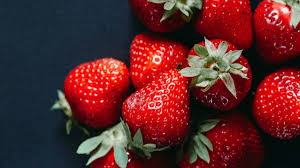
\includegraphics[width=\textwidth]{Figures/fruit1.jpeg}
    \caption{First subfigure.}
    \label{fig:first}
\end{subfigure}
\hfill
\begin{subfigure}{0.4\textwidth}
    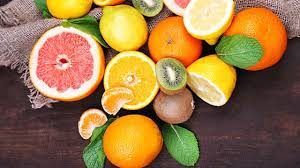
\includegraphics[width=\textwidth]{Figures/fruit2.jpeg}
    \caption{Second subfigure.}
    \label{fig:second}
\end{subfigure}
\hfill
\begin{subfigure}{0.4\textwidth}
    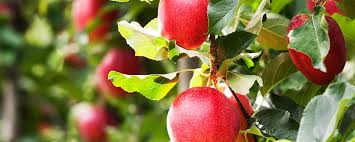
\includegraphics[width=\textwidth]{Figures/fruit3.jpeg}
    \caption{Third subfigure.}
    \label{fig:third}
\end{subfigure}
        
\caption{Creating subfigures.}
\label{fig:figures}
\end{figure}

\section{Section 2 Heading}

Contents

\subsection{Subsection Heading}

Contents
	
	\section{Summary and Gaps Identified}
	\paragraph\ 
	This is the most important section of Chapter 2. This subsection has two parts (i) summary 	and (ii) gaps identified. Summary can be a tabular form mentioning the advantages/disadvantages associated with each title. The gaps identified can be a numbered list of around four or five points mentioning what is lacking in the current state of art.
	
	Chapter conclusion goes here.
Here's a structured chapter in the form of **System Architecture** with sections and subsections corresponding to each component you've provided:

---

\chapter{System Architecture}

This chapter describes the architecture of the system, outlining each component involved in creating an efficient demand forecasting and vendor collaboration platform. The system utilizes advanced machine learning and optimization techniques to support small-scale vendors by providing demand forecasting, order aggregation, and logistics optimization.

\section{Dataset}

The dataset is the foundation of the demand forecasting model, containing historical sales data at the store-item level. This data enables the platform to make informed predictions and optimizations.

\section{Preprocessing}

Data preprocessing is crucial to ensure that the dataset is clean, consistent, and ready for model training. This step includes handling missing values, standardizing date formats, and splitting data into training and testing sets.

\section{Feature Extraction}

Feature extraction involves deriving additional information from raw data to improve the model’s predictive accuracy. The platform applies various feature engineering techniques to capture meaningful patterns in the dataset.

\subsection{Time-Based Features}

Time-based features include day-of-week, month, season, and holiday indicators. These features help capture temporal patterns and seasonality, which are important in predicting demand trends.

\subsection{Lagged Variables}

Lagged variables capture dependencies between current sales and past sales. These features are essential for understanding demand fluctuations and for integrating historical patterns into the forecasting model.

\section{Demand Forecasting with Neural Prophet}

Demand forecasting is achieved using the Neural Prophet model, which incorporates seasonality, trend components, and other covariates. This section outlines the implementation and configuration of the model to predict future sales.

\section{Order Aggregation using Genetic Algorithm}

Order aggregation is an optimization process using a Genetic Algorithm to combine multiple vendor orders. The aim is to meet minimum order quantities (MOQs) and maximize cost savings through bulk purchasing.

\section{Logistics Optimization with Green Routing}

The system’s logistics optimization uses Green Routing techniques to reduce transportation costs and minimize environmental impact. This section details the two main components of the routing optimization.

\subsection{Path Flexibility}

Path flexibility allows for alternative routes within delivery schedules. It ensures efficiency in logistics by adapting routes to current traffic conditions and delivery requirements.

\subsection{Service Time Window}

Service time windows define acceptable delivery times for each location. This feature ensures timely delivery while optimizing route scheduling to meet vendor and customer needs.

\section{Model Evaluation and Optimization}

Model evaluation is performed using metrics like Mean Absolute Error (MAE) and Root Mean Square Error (RMSE) to ensure accurate predictions. Optimization steps are undertaken to enhance model performance.

\subsection{Evaluation}

This step involves assessing the model's accuracy and performance on validation data. Evaluation metrics help identify areas for improvement in the forecasting model.

\subsection{Hyperparameter Tuning}

Hyperparameter tuning uses techniques like grid search to optimize model parameters. The goal is to enhance prediction accuracy and generalization to new data.

\subsection{Iterative Optimization}

An iterative optimization process allows the model to continuously improve by refining feature engineering and adjusting model parameters based on feedback from performance metrics.

\section{System Integration and Notifications}

The system integrates each component to ensure seamless data flow and effective communication between users. Notifications inform vendors about important updates, such as order status, inventory levels, and delivery schedules.

\par 
This chapter has outlined the system architecture, providing a detailed view of each component’s role in the platform's functionality. Together, these components create a cohesive system that supports demand forecasting, order aggregation, and efficient logistics management for vendors.

--- 

This structure integrates your sections and subsections while describing their purpose in the system's context. Let me know if you’d like additional details in any section!
\chapter{DESIGN AND MODELING}

Design and modeling are essential phases in the software development lifecycle, playing a
crucial role in the creation of effective and wellstructured systems. These phases involve
the conceptualization, planning, and representation of a software solution before its actual
implementation.
\section{Activity Diagram}
An activity diagram is a type of UML (Unified Modeling Language) diagram that visually represents the flow of activities in a system or business process. It is commonly used in software development to illustrate the dynamic aspects of a system and describe how different activities or tasks interact with each other. Activity diagrams are particularly useful for modeling the workflow within a system and for understanding the sequence of actions that take place.

\subsection{Key elements of Activity Diagrams}
\begin{itemize}
    \item \textbf{Activity:} Represented by rounded rectangles, activities are the specific tasks or actions that are performed within the system. These can range from simple operations to complex processes.
    \item \textbf{Transitions:} Arrows connecting activities indicate the flow or transition from one activity to another. The direction of the arrow shows the order of execution.
    \item \textbf{Decision Nodes:} Diamonds are used to represent decision points in the workflow. Depending on certain conditions, the process may take different paths.
    \item \textbf{Fork and Join Nodes:} Fork nodes (split) and join nodes (merge) show parallel or concurrent activities. Forks represent the divergence of multiple flows, while joins represent their convergence.
    \item \textbf{Initial and Final Nodes:} Circles are used to denote the start (initial node) and end (final node) of the activity diagram. The initial node represents the beginning of the process, and the final node indicates the conclusion.
\end{itemize}


\begin{figure}[H]
    \centering
    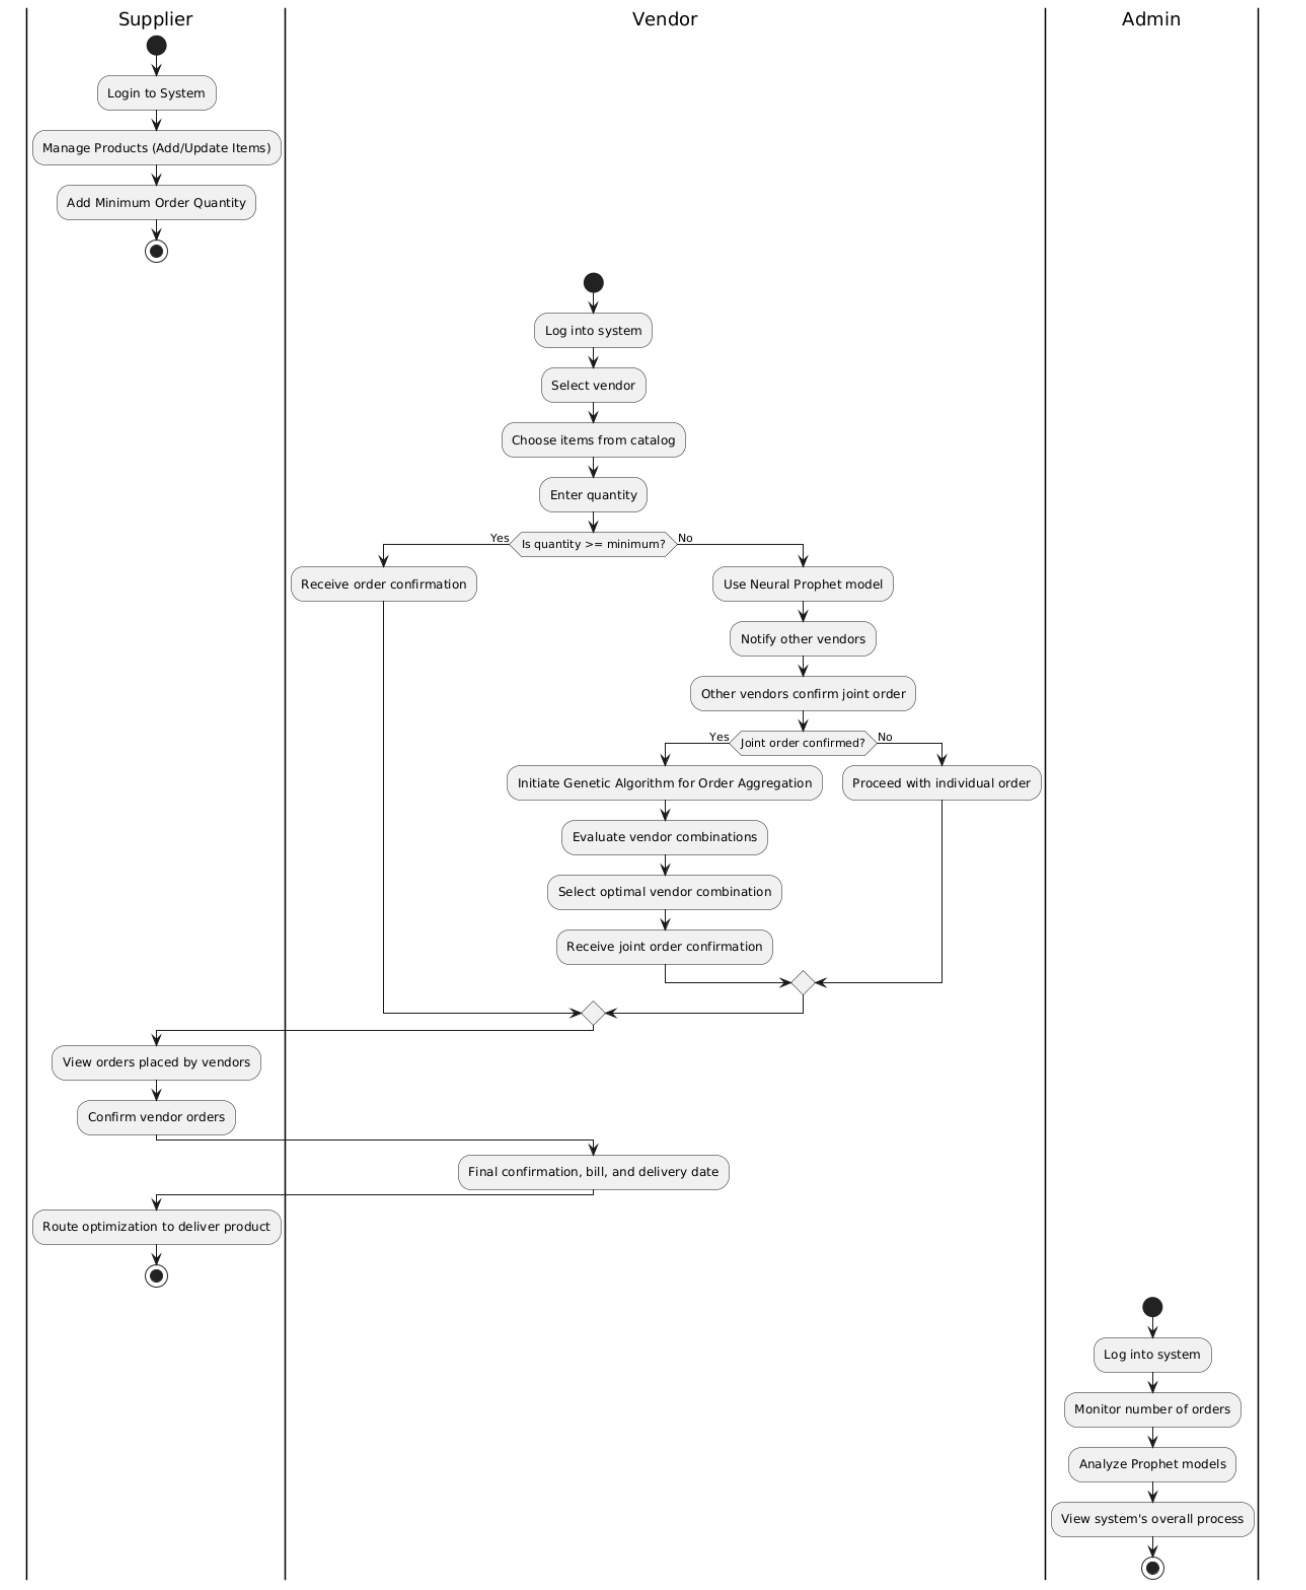
\includegraphics[width=0.9\textwidth]{Figures/Activity diagram.jpeg}
    \caption{Activity Diagram}
    \label{fig:activity-diagram}
\end{figure}
\noindent Figure 4.1 illustrates the activity diagram for the ASTRO Platform, showcasing the sequence of activities performed by suppliers, vendors, and admins. This diagram provides a high-level overview of the key entities and components involved in the system, detailing their interactions and responsibilities throughout the order processing and delivery process.

\subsection{Key Entities and Components}
\begin{enumerate}
    \item \textbf{Supplier Activities}
          \begin{enumerate}
              \item \textbf{Login to System:} The supplier logs into the system to access functionalities for managing products and tracking orders.
              \item \textbf{Manage Products (Add/Update Items):} Suppliers add or update product listings to ensure the catalog is up-to-date and accurate.
              \item \textbf{Add Minimum Order Quantity:} Suppliers set a minimum order quantity for each product, preventing inefficient processing of very small orders.
              \item \textbf{View Orders Placed by Vendors:} Suppliers can view pending orders from vendors, preparing them for order fulfillment.
              \item \textbf{Confirm Vendor Orders:} Suppliers review and confirm vendor orders, moving them to the fulfillment phase.
              \item \textbf{Route Optimisation for Delivery:} The supplier optimizes delivery routes to reduce logistics costs and ensure timely product delivery.
          \end{enumerate}

    \item \textbf{Vendor Activities}
          \begin{enumerate}
              \item \textbf{Log into System:} Vendors start by logging into the system to access the product catalog and ordering functionalities.
              \item \textbf{Select Vendor and Choose Items from Catalog:} Vendors select suppliers to order from, browsing the catalog to choose items.
              \item \textbf{Enter Quantity:} Vendors input desired quantities for each item, triggering a check against the minimum order quantity.
              \item \textbf{Quantity Check (Yes/No):}
                    \begin{itemize}
                        \item \textbf{If Quantity Meets Minimum Requirement:} The order is confirmed directly.
                        \item \textbf{If Quantity Is Below Minimum Requirement:}
                              \begin{enumerate}
                                  \item \textbf{Use Neural Prophet Model:} The system uses a Neural Prophet model to forecast demand and determine if combining orders with other vendors can reach the minimum order threshold.
                                  \item \textbf{Notify Other Vendors:} Other vendors are notified to consider joining a joint order.
                                  \item \textbf{Joint Order Confirmation Check (Yes/No):}
                                        \begin{itemize}
                                            \item \textbf{If Other Vendors Agree:} The joint order is confirmed.
                                            \item \textbf{If Not:} The vendor proceeds with an individual order.
                                        \end{itemize}
                                  \item \textbf{Initiate Genetic Algorithm for Order Aggregation:} The system uses a genetic algorithm to identify the best vendor combinations for the joint order.
                                  \item \textbf{Evaluate Vendor Combinations:} Different combinations are assessed to find an optimal one that meets requirements.
                                  \item \textbf{Select Optimal Vendor Combination:} The system selects the optimal vendor combination, and a joint order confirmation is received.
                                  \item \textbf{Receive Final Confirmation:} Vendors receive the final confirmation, including billing details and delivery date.
                              \end{enumerate}
                    \end{itemize}
          \end{enumerate}

    \item \textbf{Admin Activities}
          \begin{enumerate}
              \item \textbf{Log into System:} The admin logs into the system to monitor and analyze overall processes.
              \item \textbf{Monitor Number of Orders:} Admin tracks order volumes, gaining insights into demand trends and operational load.
              \item \textbf{Analyze Prophet Models:} Admin reviews the performance of demand forecasting models, such as Neural Prophet, to ensure accurate predictions and make adjustments if necessary.
              \item \textbf{View System's Overall Process:} Admin has a top-down view of system activities to ensure smooth operations and identify areas for improvement.
          \end{enumerate}
\end{enumerate}


Here’s how activity diagrams can be specifically helpful in this context:
\begin{itemize}
    \item Enhanced Clarity of Process Flow: The diagram visually represents the process, making it easier for stakeholders to understand each role's responsibilities and interactions. By defining the steps each role follows, the diagram ensures that all parties (Suppliers, Vendors, and Admins) understand their tasks and when each task needs to be completed.
    \item Identification of Key Decision Points: The activity diagram highlights critical decision points, such as the quantity check for minimum orders. This helps in identifying points where conditional logic and alternative flows come into play, ensuring that the system can handle various scenarios efficiently. For example, if the order quantity is insufficient, the system automatically checks for joint orders, thus streamlining the process without manual intervention.
    \item Improved Coordination Between Roles: By detailing the interactions between suppliers, vendors, and admins, the diagram promotes better coordination. Vendors can initiate joint orders when quantities are low, and suppliers can confirm orders and optimize delivery routes accordingly. This collaboration ensures that orders are fulfilled more efficiently and that each role's activities are synchronized.
    \item Guidance for System Design and Development: For developers, the activity diagram serves as a blueprint for creating system modules. Each activity can be mapped to specific features in the system, like order confirmation, joint order aggregation, route optimisation, and demand forecasting using the Neural Prophet model. This structured approach helps in modular and organized system development, making the codebase easier to manage and maintain.
\end{itemize}
\section{Sequence Diagram}

A sequence diagram is a type of UML (Unified Modeling Language) diagram that illustrates the interactions between different components or actors in a system over time. It presents a chronological sequence of messages or actions between the various entities, providing a visual representation of the dynamic behavior of the system.
\subsection{Key elements of Sequence Diagrams}

\begin{itemize}
    \item \textbf{Actors and Objects:} Represent the entities (users, systems, or objects) involved in the interactions.
    \item \textbf{Lifelines:} Vertical lines extending from actors or objects, showing their presence over time in the sequence.
    \item \textbf{Messages:} Arrows that represent the communication between lifelines, including method calls, data exchanges, and responses.
    \item \textbf{Activation Bars:} Narrow rectangles on lifelines indicating when an object is actively performing a task.
    \item \textbf{Control Structures:} Elements like loops, conditions, and alternative frames (alt/opt frames) that model conditional, repeated, or optional interactions.
    \item \textbf{Destruction:} Marked by an "X" at the end of a lifeline, indicating the termination of an object in the sequence.
\end{itemize}
\subsection{Purpose of Sequence Diagrams}
\begin{itemize}
    \item {Understanding System Behavior:} Sequence diagrams help in understanding how different components or actors in a system interact with each other over time, depicting the flow of control and communication.
    \item {Communication:} They serve as a communication tool among stakeholders, including developers, designers, and project managers, by offering a clear and visual representation of system interactions.
    \item {Design and Analysis:} Sequence diagrams aid in the design and analysis phases of software development, helping to identify potential issues in the system’s logic or communication flow.
    \item {Visualizing the Workflow:} It provides a clear and concise overview of the different steps involved in the Alzheimer’s disease detection process.
    \item {Identifying Potential Bottlenecks:} It helps to identify any potential bottlenecks in the system, such as slow preprocessing steps or inaccurate model predictions.
    \item {Facilitating Communication:} It serves as a common language for developers, researchers, and other stakeholders involved in the project.
\end{itemize}

\begin{figure}[H]
    \centering
    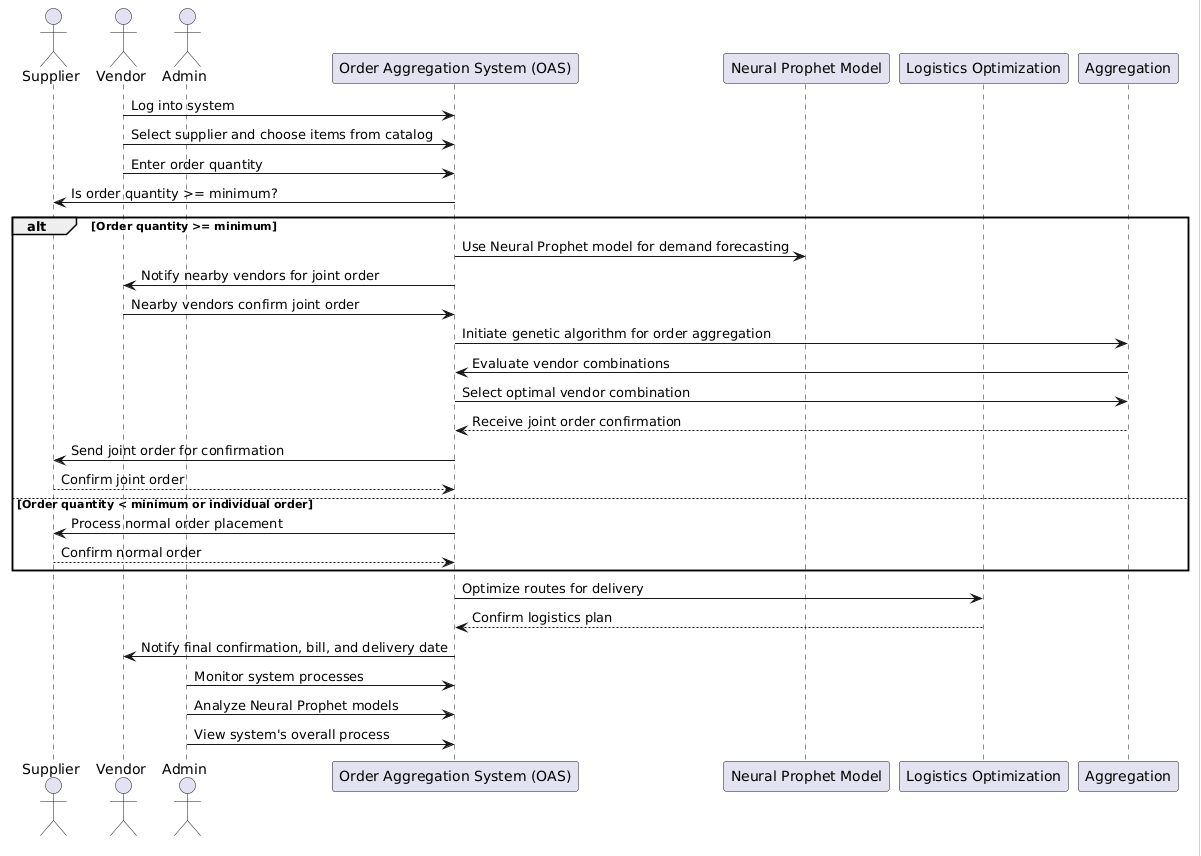
\includegraphics[width=1\textwidth]{Figures/Sequence Diagram.PNG}
    \caption{Sequence Diagram}
    \label{fig:sequence-diagram}
\end{figure}
\noindent Figure 4.2 illustrates the sequence of interactions between the key entities and components of the ASTRO Platform. This diagram provides a step-by-step view of how the system processes an order from initiation to delivery. It shows the flow of messages and the order in which they are exchanged, highlighting the interactions between the Supplier, Vendor, Admin, Order Aggregation System (OAS), Neural Prophet Model, and Logistics Optimisation.
\subsection{Key Entities and Components}
\begin{itemize}
    \item \textbf{Supplier:} Manages product inventory and fulfills confirmed orders.
    \item \textbf{Vendor:} Places orders for products based on the demand forecast and minimum order requirements.
    \item \textbf{Admin:} Monitors the overall process, analyzes model performance, and reviews logistics planning.
    \item \textbf{Order Aggregation System (OAS):} Core system component that manages the flow of order requests, checks conditions, and coordinates with other components.
    \item \textbf{Neural Prophet Model:} A demand forecasting model that helps in predicting demand and evaluating whether joint orders would be beneficial.
    \item \textbf{Logistics Optimisation:} Component responsible for optimizing delivery routes and managing the final logistics.
\end{itemize}
\subsection{Sequence of Interactions}

\begin{enumerate}
    \item \textbf{Login to System:} The Vendor initiates the sequence by logging into the system to access the product catalog, choose items, and place orders.
    \item \textbf{Select Supplier and Choose Items from Catalog:} The Vendor selects a supplier and items from the catalog, specifying the order quantity.
    \item \textbf{Order Quantity Check:} The Order Aggregation System (OAS) checks whether the order quantity meets the minimum order requirement.
          \begin{itemize}
              \item \textbf{If Order Quantity Meets Minimum Requirement:} The order is processed as a standard, individual order. The vendor confirms the order, and it proceeds to the delivery logistics phase.
              \item \textbf{If Order Quantity Is Below Minimum Requirement:} The OAS initiates steps to evaluate the feasibility of a joint order.
                    \begin{enumerate}
                        \item \textbf{Use Neural Prophet Model for Demand Forecasting:} The Neural Prophet Model is used to forecast demand and determine if combining orders from nearby vendors might help reach the minimum order quantity. This forecast provides data-driven insights into the order’s potential demand over time.
                        \item \textbf{Notify Nearby Vendors for Joint Order:} If the demand forecast suggests that a joint order is viable, the OAS sends notifications to nearby vendors, inviting them to participate in a joint order.
                        \item \textbf{Nearby Vendors Confirm Joint Order:} Other vendors respond to the joint order request. If they agree, the joint order process moves forward; otherwise, the initial vendor proceeds with an individual order.
                        \item \textbf{Initiate Genetic Algorithm for Order Aggregation:} The OAS employs a Genetic Algorithm to evaluate different combinations of vendors for the joint order, aiming to find an optimal mix that maximizes efficiency and meets the minimum order requirements.
                        \item \textbf{Evaluate Vendor Combinations:} The Genetic Algorithm component iterates through various vendor combinations to find the best possible aggregation. This ensures that the order is cost-effective and meets quantity requirements.
                        \item \textbf{Select Optimal Vendor Combination:} The system selects the optimal vendor combination for the joint order and proceeds to confirmation.
                        \item \textbf{Receive Joint Order Confirmation:} Once an optimal combination is selected, the OAS sends a joint order confirmation to all participating vendors. The joint order is now officially confirmed.
                    \end{enumerate}
          \end{itemize}
    \item \textbf{Order Processing and Final Confirmation:} For both joint and individual orders, the system notifies vendors of the final confirmation, bill, and delivery date.
    \item \textbf{Optimize Routes for Delivery:} The Logistics Optimisation component optimizes delivery routes based on the confirmed orders, minimizing delivery time and cost by consolidating deliveries where possible.
    \item \textbf{Admin Activities:} The Admin monitors system processes and performance. Admin also reviews and analyzes the accuracy of Neural Prophet Model forecasts and evaluates system functionality, using insights to make improvements to the process.
\end{enumerate}
\section{Class Diagram}

A class diagram is a visual blueprint of a system in object-oriented programming, showcasing the classes, their attributes (properties), operations (methods), and the relationships between them. It’s like a map that reveals the building blocks and their connections, guiding the development and understanding of the system.

\subsection{Key Elements of Class Diagrams}
\begin{itemize}
    \item \textbf{Classes:} These are the fundamental building blocks, represented as rectangles with the class name inside. Each class encapsulates a specific concept or entity within the system, like "Customer" or "Order."
    \item \textbf{Attributes:} These define the data associated with a class, like "name" and "address" for the "Customer" class. They’re listed within the class rectangle, often with data types specified.
    \item \textbf{Operations:} These represent the actions a class can perform, like "placeOrder" or "calculateTotal" for the "Order" class. They’re shown as functions within the class rectangle, with their parameters and return values if applicable.
    \item \textbf{Relationships:} These depict the connections between classes, indicating how they interact with each other.
\end{itemize}
\begin{figure}[H]
    \centering
    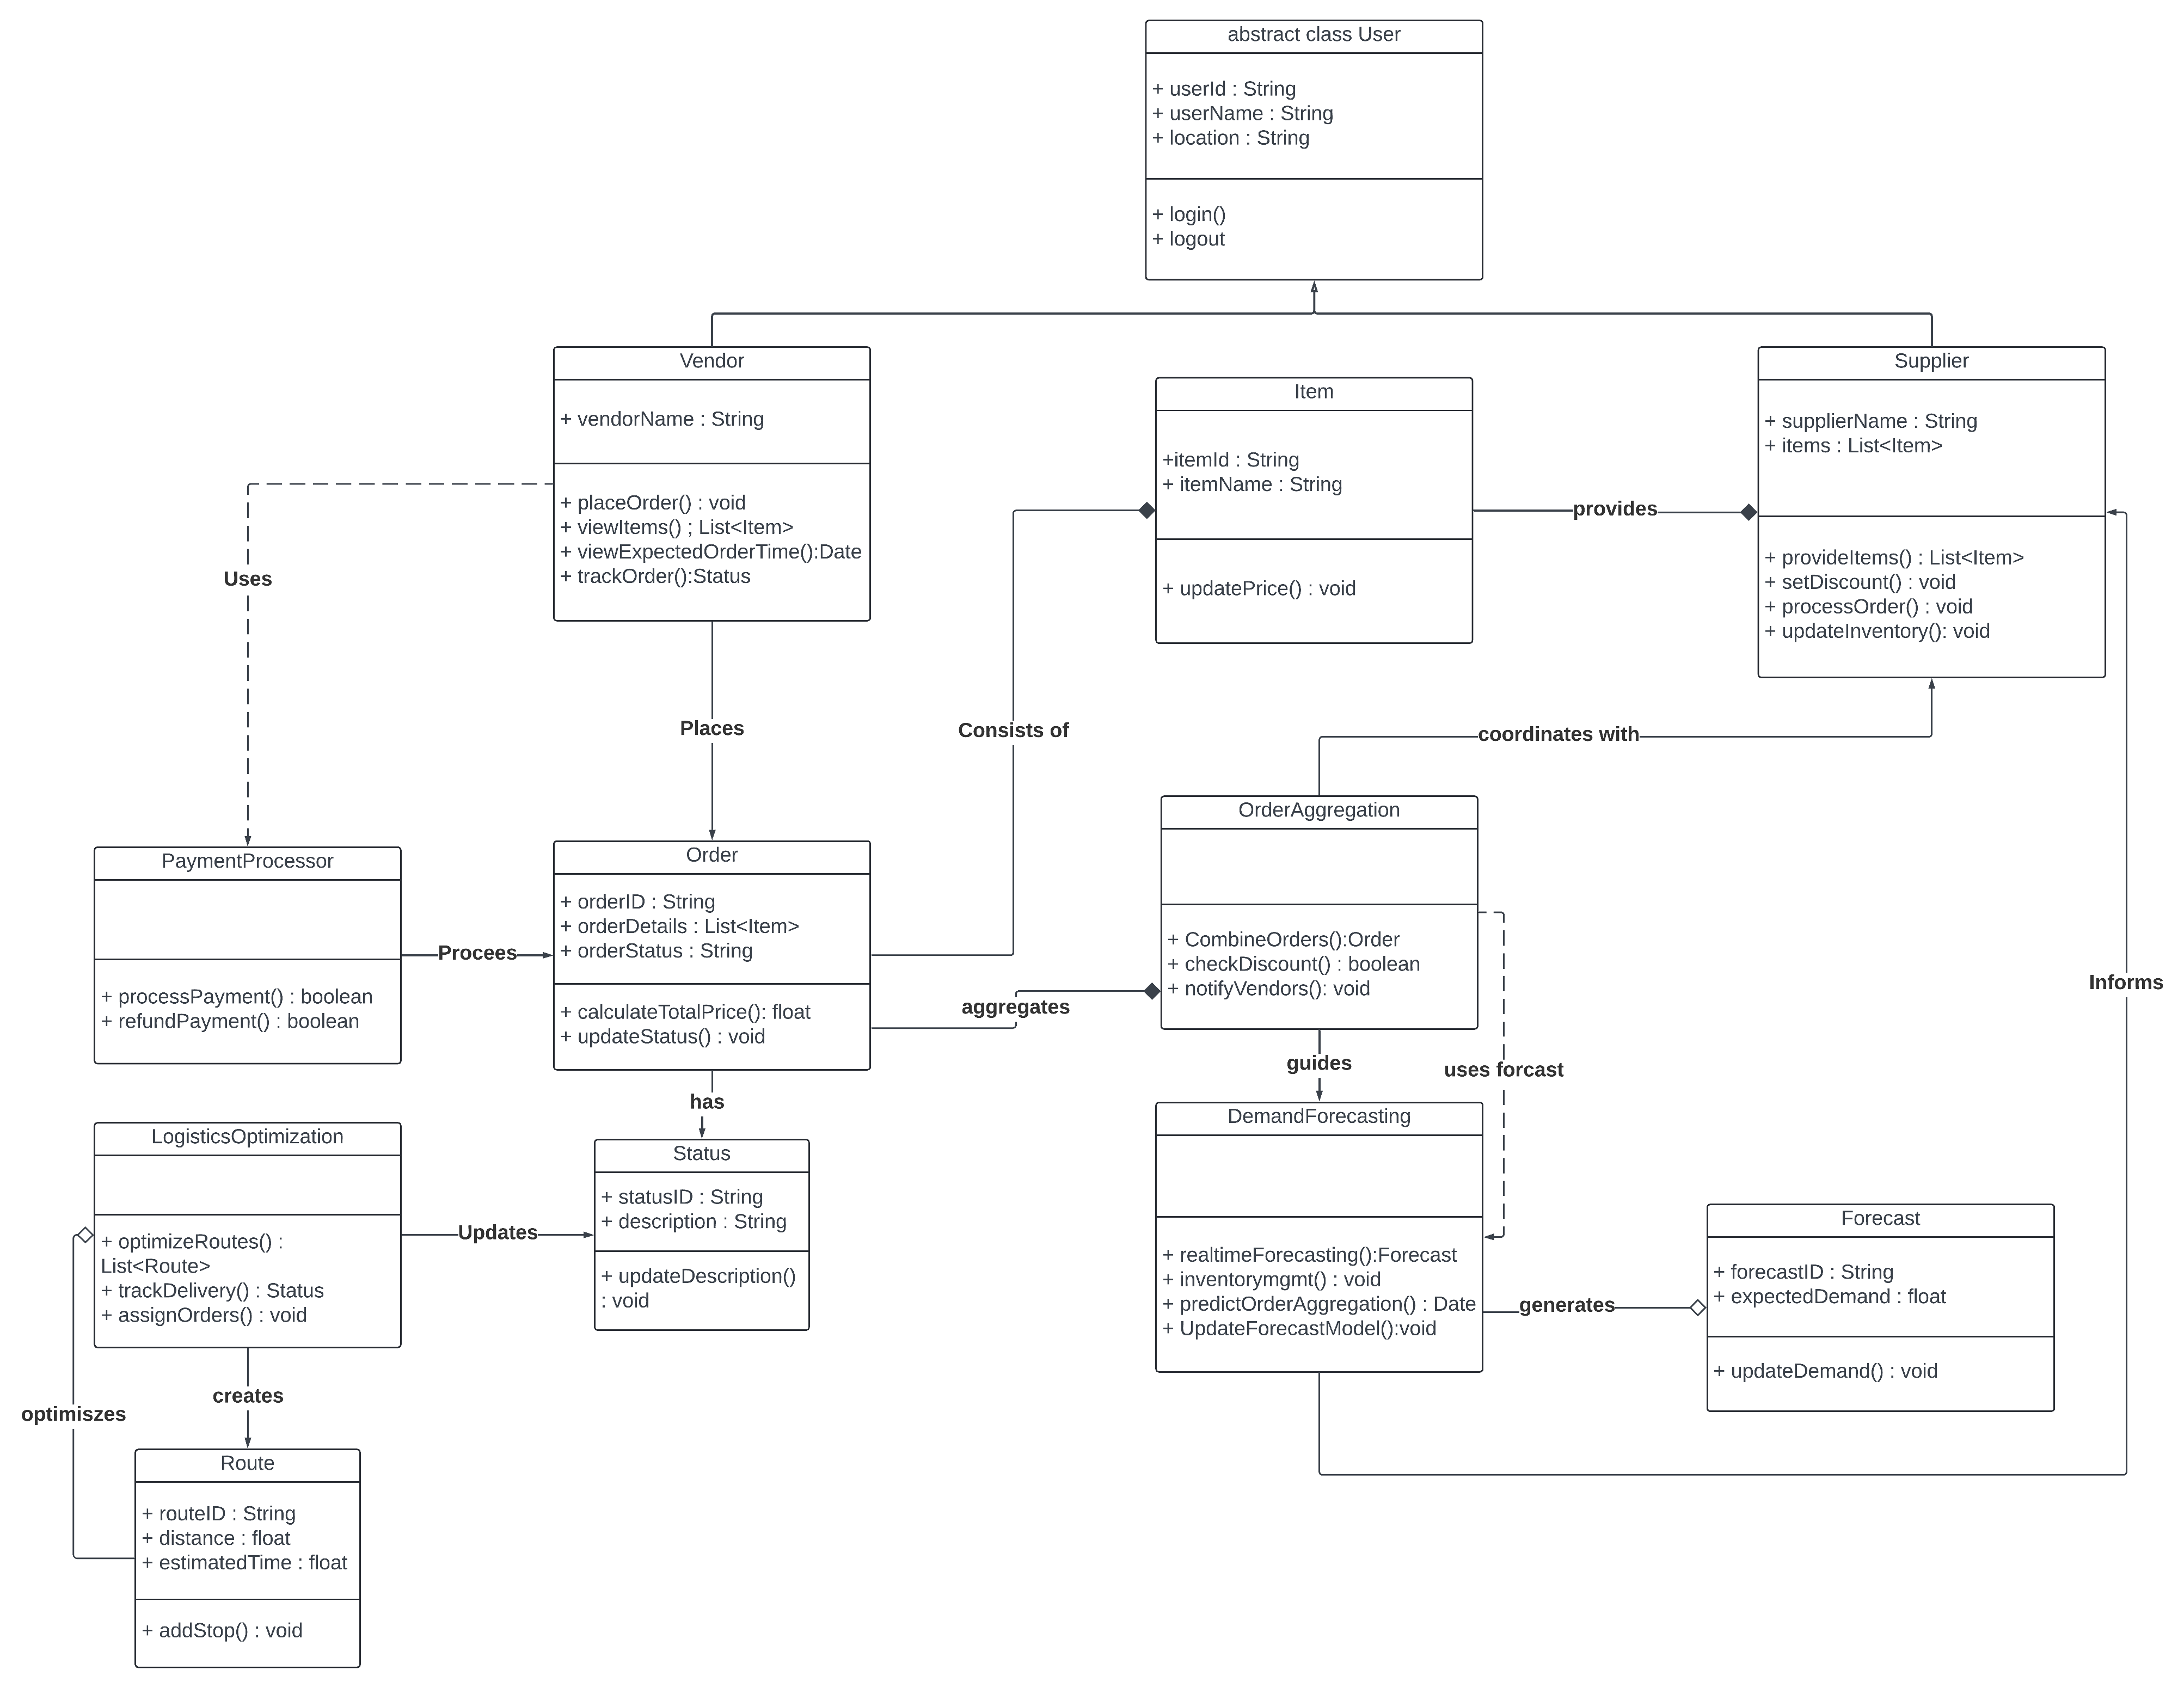
\includegraphics[width=1\textwidth]{Figures/Class Diagram.png}
    \caption{Class Diagram}
    \label{fig:class-diagram}
\end{figure}
\noindent Figure 4.3 illustrates the class diagram for the ASTRO Platform, showcasing the key classes and their relationships. This diagram provides a structural overview of the system, detailing the classes like User, Vendor, Supplier, Item, Order, Status, OrderAggregation, PaymentProcessor, LogisticsOptimization, DemandForecasting, and Forecast, along with their attributes and methods.
\subsection{Class Descriptions}

\begin{itemize}
    \item \textbf{User:} An abstract class representing a generic user with attributes like userId, userName, and location, along with methods login() and logout(). Inherited by Vendor and Supplier classes.

    \item \textbf{Vendor:} Represents a vendor who manages orders, with attributes such as vendorName and methods like placeOrder(), viewItems(), viewExpectedOrderTime(), and trackOrder(). Associated with Order and interacts with PaymentProcessor for payment handling.

    \item \textbf{Supplier:} Represents a supplier managing inventory with attributes like supplierName and items, and methods like provideItems(), setDiscount(), processOrder(), and updateInventory(). Coordinates with OrderAggregation and supplies items to the Item class.

    \item \textbf{Item:} Represents individual items with attributes like itemId and itemName, and a method updatePrice() to modify the item's price. Associated with Order as orders consist of multiple items.

    \item \textbf{Order:} Represents a customer order, including attributes orderID, orderDetails (list of items), and orderStatus, with methods calculateTotalPrice() and updateStatus(). Consists of multiple Item objects and is associated with Status.

    \item \textbf{Status:} Represents the order's current status with attributes statusID and description, and a method updateDescription() to modify the status description. Linked to Order to provide status details.

    \item \textbf{OrderAggregation:} Manages combined orders with methods CombineOrders(), checkDiscount(), and notifyVendors(). Coordinates with Supplier for order processing and informs DemandForecasting about aggregate demand.

    \item \textbf{PaymentProcessor:} Handles payments and refunds with methods processPayment() and refundPayment(). Interacts with Vendor for transaction management.

    \item \textbf{LogisticsOptimization:} Optimizes delivery routes with methods optimizeRoutes(), trackDelivery(), and assignOrders(), creating Route objects as part of logistics planning.

    \item \textbf{Route:} Represents a delivery route with attributes routeID, distance, and estimatedTime, and a method addStop() to add stops. Created by LogisticsOptimization.

    \item \textbf{DemandForecasting:} Predicts demand and manages inventory with methods like realtimeForecasting(), inventoryMgmt(), predictOrderAggregation(), and updateForecastModel(). Uses data from Forecast to guide order aggregation and inventory planning.

    \item \textbf{Forecast:} Provides demand forecasts with attributes forecastID and expectedDemand, and a method updateDemand(). Generated by DemandForecasting and used for planning inventory and order aggregation.
\end{itemize}
\subsection{Summary of Associations}
\begin{enumerate}
    \item Vendor places orders using Order and interacts with PaymentProcessor.
    \item Supplier provides Items to the system and coordinates with OrderAggregation for bulk orders.
    \item OrderAggregation combines orders and coordinates with Supplier, also informing DemandForecasting.
    \item DemandForecasting uses forecasts from Forecast to plan inventory and order aggregation.
    \item LogisticsOptimization creates Routes to optimize delivery.
\end{enumerate}

\subsection{Common Relationships}
\begin{itemize}
    \item \textbf{Association:} Shows a simple connection between two classes, like "Customer" has an "Order."
    \item \textbf{Aggregation:} A "has-a" relationship where one class (the whole) is made up of parts (the other class), like "Order" has "OrderItems."
    \item \textbf{Composition:} A stronger "has-a" relationship where the parts (the other class) cannot exist independently of the whole (one class), like "Car" has "Wheels."
    \item \textbf{Inheritance:} Shows a hierarchical relationship where one class (subclass) inherits properties and methods from another class (superclass), like "Employee" inherits from "Person."
\end{itemize}

\subsection{Benefits of Using Class Diagrams}
\begin{itemize}
    \item \textbf{Clarity:} They provide a visual representation of complex systems, making them easier to understand and communicate.
    \item \textbf{Communication:} They serve as a common language for developers, designers, and other stakeholders to agree on the system’s structure.
    \item \textbf{Analysis:} They help identify potential problems or inconsistencies in the system’s design before implementation.
    \item \textbf{Documentation:} They serve as a valuable reference for understanding and maintaining the system over time.
\end{itemize}

Where You Might Encounter Them
\begin{itemize}
    \item \textbf{Software Development:} Class diagrams are used throughout the software development lifecycle, from initial design to implementation and maintenance.
    \item \textbf{System Design:} They are crucial for modeling the architecture of complex systems, including web applications and enterprise software.
    \item \textbf{Documentation:} They are often included in technical documentation to provide a clear overview of the system’s structure.
\end{itemize}
\section{Use Case Diagram}
In the Unified Modeling Language (UML), a Use Case Diagram is a sort of behavioral diagram that depicts the interactions between various actors (users or external systems) and a system that is being studied. It offers a high-level perspective on how different entities use the features or functionalities of a system. A use case diagram’s main objective is to represent and illustrate the various ways users engage with a system and the results they receive.
\subsection{Key Elements of Use Case Diagrams}

\begin{itemize}
    \item \textbf{Use Case:} A use case is an example of a particular functionality or group of related functions that the system offers to its users, also known as actors. Use cases are designated to indicate a particular action or objective and are usually represented as ovals.

    \item \textbf{Actor:} An outside party interacting with the system is called an actor. Actors might be physical devices, other systems, or human actors. Stick figures are used to represent actors, who engage with the system by taking part in one or more use cases.

    \item \textbf{System Boundary:} Depicted as a box, the system boundary establishes the parameters of the system and demarcates its external participants. Actors reside outside the system boundaries, whereas use cases exist inside it.

    \item \textbf{Association:} Associations are shown as lines joining actors to use cases. These lines show that an actor participates in or communicates with a certain use case. Associations serve as a channel of communication between the use case and the actor.

    \item \textbf{Include Relationship:} An include relationship shows that one use case incorporates the functionality of another use case. It is represented by a dashed arrow. It suggests that the behavior of the base use case includes the added use case.

    \item \textbf{Extend Relationship:} An extended connection shows that, under certain circumstances, one use case can extend the behavior of another use case. It is represented by a dashed arrow with an open arrowhead. It suggests that the expanding use case is called upon under particular circumstances and is optional.

\end{itemize}
Some use cases might not include interactions with a particular actor; instead, they might represent system-wide operations or processes. We call these use cases for the system.

\subsection{Value of Use Case Diagrams}

Use Case Diagrams are valuable tools for:
\begin{itemize}
    \item \textbf{Communication:} Use case diagrams offer a visual representation that helps stakeholders—developers, designers, and non-technical stakeholders—communicate with one other.
    \item \textbf{Requirements Analysis:} By recognizing and recording user-system interactions, they aid in the elicitation and clarification of system requirements.
    \item \textbf{System Design:} The architecture and user interfaces of the system are designed using use case diagrams as a guide.
    \item \textbf{Testing:} By figuring out scenarios in which users engage with the system, they can be used to generate test cases.
    \item \textbf{Project Planning:} By highlighting important features and their relationships, use case diagrams can help with project planning.
\end{itemize}
\begin{figure}[H]
    \centering
    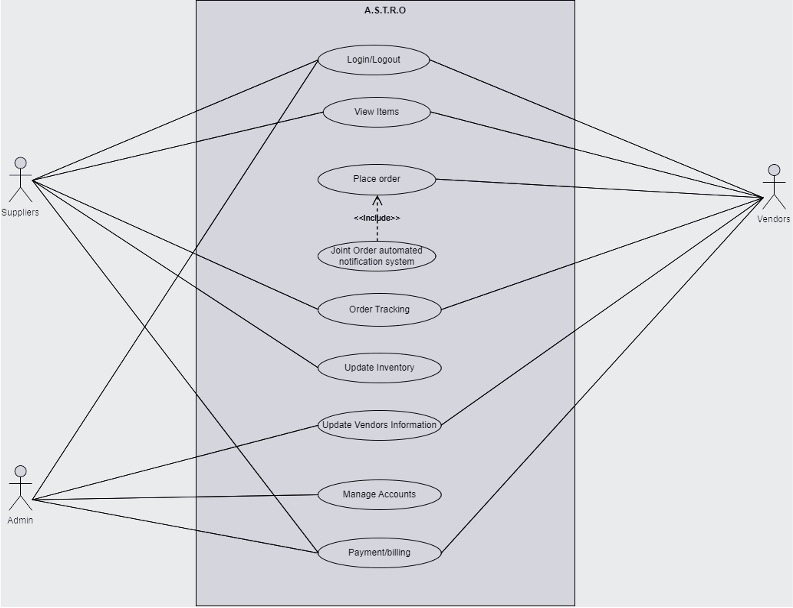
\includegraphics[width=1\textwidth]{Figures/Use case diagram.jpg}
    \caption{Use Case Diagram}
    \label{fig:use-case-diagram}
\end{figure}
\noindent Figure 4.4 illustrates the use case diagram for the ASTRO Platform, showcasing the interactions between the actors (Suppliers, Vendors, and Admin) and the system. This diagram provides a high-level view of the functionalities available to each actor and how they interact with the system to place orders, manage inventory, track orders, and perform administrative tasks.
\subsection{Actors}

\begin{enumerate}
    \item \textbf{Suppliers:}
          \begin{itemize}
              \item Responsible for providing inventory or items for the system.
              \item Has access to most functions related to orders, inventory, and tracking.
          \end{itemize}

    \item \textbf{Vendors:}
          \begin{itemize}
              \item Likely responsible for purchasing or receiving items in the system.
              \item Similar to Suppliers, has access to most functions, especially those related to placing orders, notifications, and tracking.
          \end{itemize}

    \item \textbf{Admin:}
          \begin{itemize}
              \item Responsible for overall management, including accounts and billing.
              \item Has the ability to manage vendor information and accounts in addition to other functionalities.
          \end{itemize}
\end{enumerate}
\subsection{Use Cases}

\begin{enumerate}
    \item \textbf{Login/Logout:}
          \begin{itemize}
              \item All users (Suppliers, Vendors, and Admin) can log in and log out of the system, indicating that authentication is a standard feature.
          \end{itemize}

    \item \textbf{View Items:}
          \begin{itemize}
              \item Suppliers and Vendors have access to this use case, allowing them to view items available in the system, possibly for ordering or tracking purposes.
          \end{itemize}

    \item \textbf{Place Order:}
          \begin{itemize}
              \item Both Suppliers and Vendors can place orders in the system, which might include ordering goods or services. This use case includes an include relationship to the Joint Order Automated Notification System use case, meaning that when an order is placed, an automated notification system is triggered.
          \end{itemize}

    \item \textbf{Joint Order Automated Notification System:}
          \begin{itemize}
              \item An included use case for the Place Order use case.
              \item This automated system sends notifications for joint orders, possibly to inform both Suppliers and Vendors of order status or details.
          \end{itemize}

    \item \textbf{Order Tracking:}
          \begin{itemize}
              \item Both Suppliers and Vendors can track the status of their orders through the system, giving them visibility into order fulfillment stages.
          \end{itemize}

    \item \textbf{Update Inventory:}
          \begin{itemize}
              \item This use case allows both Suppliers and Vendors to update inventory information, which could involve adding, editing, or removing items based on stock levels or requirements.
          \end{itemize}

    \item \textbf{Update Vendors Information:}
          \begin{itemize}
              \item Accessible by all actors, including Admin.
              \item This use case allows updating information related to Vendors, which could involve updating contact details, address, or other essential information.
          \end{itemize}

    \item \textbf{Manage Accounts:}
          \begin{itemize}
              \item Specific to the Admin, who has control over managing accounts in the system.
              \item This might involve user account creation, permissions, and other administrative tasks.
          \end{itemize}

    \item \textbf{Payment/Billing:}
          \begin{itemize}
              \item Only the Admin has access to this functionality, likely responsible for handling the financial aspects of transactions in the system, including processing payments and issuing bills.
          \end{itemize}
\end{enumerate}
\subsection{Relationships}

\begin{itemize}
    \item \textbf{Include Relationship:}
          The Place Order use case includes the Joint Order Automated Notification System, meaning that this automated notification is a required part of placing an order. This might help keep all parties informed about order updates.


    \item \textbf{System Boundary:}
          The shaded box labeled ASTRO represents the system boundary, meaning all the use cases within this box are functionalities provided by the ASTRO system.

\end{itemize}
\chapter{Conclusions \& Future Scope}

The ASTRO platform represents a comprehensive solution designed to empower small-scale vendors by addressing their core operational challenges. By facilitating collaborative purchasing, optimizing logistics, and offering data-driven financial services, ASTRO significantly enhances the competitive edge of small vendors, enabling them to compete more effectively with large retail chains. The platform’s multifaceted approach not only reduces operational costs and improves efficiency but also provides vendors with the financial resources and data insights necessary for informed decision-making and strategic growth.

Through collaborative purchasing, ASTRO enables vendors to achieve bulk pricing discounts, thereby reducing the cost of goods sold and increasing profitability. The logistics optimization feature streamlines delivery routes, minimizing transportation costs and ensuring timely deliveries, which enhances customer satisfaction and operational reliability. Additionally, the integration of data-driven financial services addresses the critical issue of limited access to capital, providing vendors with tailored credit assessments and loan options based on their transaction data. This financial support is instrumental in facilitating business expansion, inventory management, and investment in technology.

ASTRO’s real-time demand forecasting tool equips vendors with the ability to anticipate market demand accurately, optimizing inventory levels and reducing the risk of overstocking or stockouts. This predictive capability not only enhances operational efficiency but also ensures that vendors can meet customer needs promptly and effectively. The platform’s user-friendly interface ensures accessibility and ease of use, allowing vendors with varying levels of technical expertise to leverage its features effectively.

Overall, ASTRO fosters economic resilience and sustainability within local communities by empowering small-scale vendors to thrive in a competitive marketplace. By addressing the challenges of limited purchasing power, inefficient logistics, restricted financial access, and lack of data-driven decision-making, ASTRO contributes to the long-term success and stability of small vendors, promoting a more diverse and robust local economy.

While ASTRO has made significant strides in empowering small-scale vendors, there are numerous opportunities for future enhancements and expansions to further augment its impact and effectiveness. The following areas outline potential future developments:

\begin{enumerate}
    \item \textbf{Advanced Forecasting and Predictive Analytics}: Integrate more sophisticated machine learning algorithms to enhance the accuracy and granularity of demand forecasting, allowing vendors to anticipate market trends more accurately and optimize inventory management.
    \item \textbf{AI-Enhanced Credit Assessment}: Develop AI-driven credit scoring models that utilize a broader range of data points, including transaction history and purchasing patterns, to provide personalized and accurate financial services.
    \item \textbf{Integration with Broader Supply Chains}: Establish partnerships with larger suppliers and logistics providers to expand ASTRO’s logistics optimization features, enabling vendors to access a wider range of products at competitive prices.
    \item \textbf{Sustainability Initiatives}: Incorporate environmentally sustainable practices, such as carbon footprint tracking and eco-friendly route planning, to align vendors with growing consumer demand for eco-friendly products.
    \item \textbf{Customizable Vendor Portals and Data Insights}: Develop customizable dashboards for tailored analytics based on vendor-specific needs, enabling strategic business decisions.
    \item \textbf{Expansion of Financial Services}: Introduce more financial products, such as insurance and investment options, to provide vendors with comprehensive financial support.
    \item \textbf{Enhanced Collaboration Features}: Implement tools for communication and resource sharing among vendors, fostering a sense of community and mutual support.
    \item \textbf{Mobile Application Development}: Develop a dedicated mobile application for on-the-go access to ASTRO’s features, enhancing accessibility and user engagement.
    \item \textbf{Localization and Customization}: Adapt ASTRO to different regions’ specific needs and regulatory requirements, ensuring relevance across diverse contexts.
    \item \textbf{Integration with E-Commerce Platforms}: Integrate ASTRO with popular e-commerce platforms to enable seamless online ordering and sales management, expanding vendors’ market reach.
    \item \textbf{User Training and Support Programs}: Provide training programs to help vendors maximize ASTRO’s benefits, enhancing adoption and success.
    \item \textbf{Data Privacy and Security Enhancements}: Implement advanced measures for data protection, building user trust and ensuring data confidentiality.
    \item \textbf{Feedback and Continuous Improvement Mechanism}: Establish a feedback system to gather user input and improve ASTRO’s features and functionalities over time.
    \item \textbf{Scalability and Performance Optimization}: Ensure the platform’s scalability and performance can handle increased users and data as ASTRO grows.
    \item \textbf{Exploration of New Markets and Industries}: Expand ASTRO’s framework to apply to other markets and industries beyond small-scale vendors, opening new avenues for growth and impact.
\end{enumerate}





\clearpage
\renewcommand{\bibname}{References}
\addcontentsline{toc}{chapter}{References}
\bibliographystyle{IEEEtran}
\bibliography{references}
%\input{references.tex}

\clearpage
\addcontentsline{toc}{chapter}{Appendix A: Presentation}
\chapter*{}
\paragraph\
\vspace{75mm}
\begin{center}
	\textbf{\huge{Appendix A: }}
	\textbf{\huge{Presentation}}
\end{center}
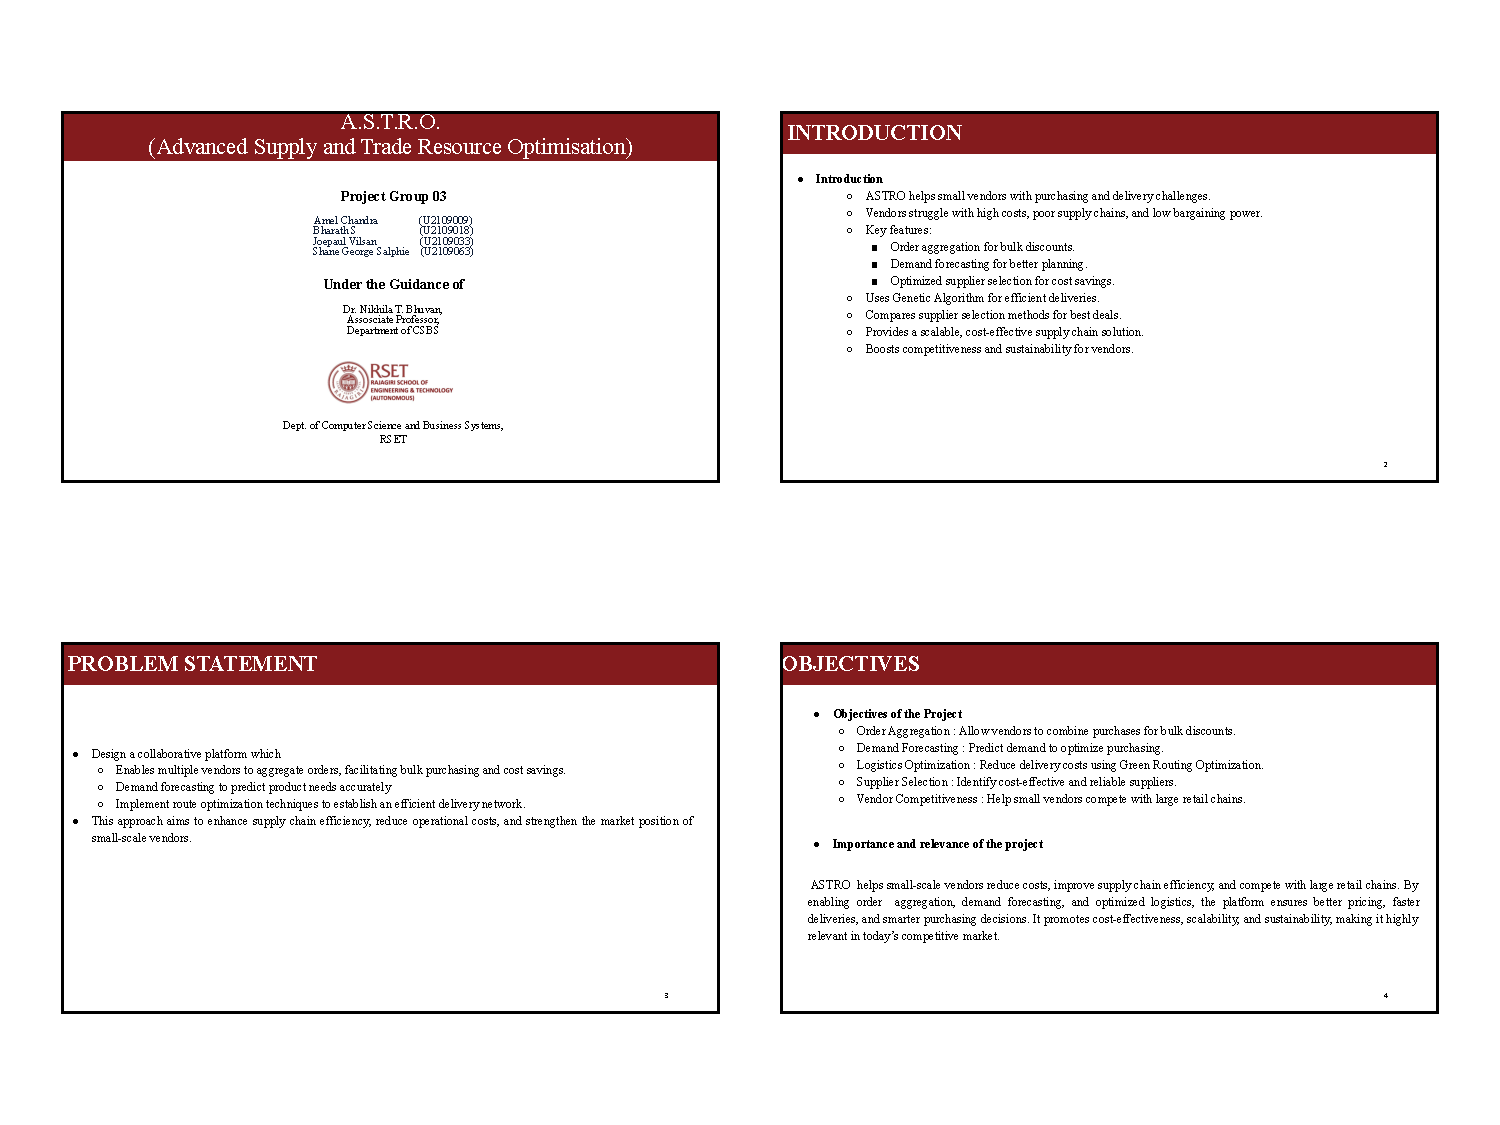
\includepdf[pages=-]{Appendices/GRP_3.pdf}

\clearpage
\addcontentsline{toc}{chapter}{Appendix B: Vision, Mission, PO, PSO, and CO}
\chapter*{}
\paragraph\
\vspace{75mm}
\begin{center}
	\textbf{\huge{Appendix B: }}
	\textbf{\huge{Vision, Mission, PO, PSO, and CO}}
\end{center}
%	\includepdf[pages=-]{2.pdf}
\clearpage
\clearpage
\newpage
%\cleardoublepage
\thispagestyle{empty}
\begin{center}
	\Large \bfseries RAJAGIRI SCHOOL OF ENGINEERING AND TECHNOLOGY (AUTONOMOUS)
\end{center}
\vspace{0.5cm}
\renewcommand{\baselinestretch}{1.2}\normalsize
\noindent\textbf{Vision}
\begin{tcolorbox}[colback=white, colframe=black, rounded corners, width=\textwidth]
	To evolve into a premier technological and research institution, molding eminent professionals with creative minds, innovative ideas and sound practical skill, and to shape a future where technology works for the enrichment of mankind.
\end{tcolorbox}

\noindent\textbf{Mission}
\begin{tcolorbox}[colback=white, colframe=black, rounded corners, width=\textwidth]
	To impart state-of-the-art knowledge to individuals in various technological disciplines and to inculcate in them a high degree of social consciousness and human values, thereby enabling them to face the challenges of life with courage and conviction.
\end{tcolorbox}

\vspace{1.5cm}
\begin{center}
	\Large \bfseries DEPARTMENT OF COMPUTER SCIENCE AND BUSINESS SYSTEMS
\end{center}
\vspace{0.5cm}
\noindent\textbf{Vision}
\begin{tcolorbox}[colback=white, colframe=black, rounded corners, width=\textwidth]
	To evolve into a department of excellence in information technology by the creation and exchange of knowledge through leading-edge research, innovation and services, which will in turn contribute towards solving complex societal problems and thus building a peaceful and prosperous mankind.
\end{tcolorbox}

\noindent\textbf{Mission}
\begin{tcolorbox}[colback=white, colframe=black, rounded corners, width=\textwidth]
	To impart high-quality technical education, research training, professionalism and strong ethical values in the young minds for ensuring their productive careers in industry and academia so as to work with a commitment to the betterment of mankind.

\end{tcolorbox}


%	To inspire and nurture students, with up-to-date knowledge in Computer Science and Engineering, ethics, team spirit, leadership abilities, innovation and creativity to come out with solutions meeting societal needs. \\ \\
\newpage
\noindent\textbf{Programme Outcomes (PO)} \\
Engineering Graduates will be able to:
\begin{enumerate}
	\item {Engineering Knowledge:} Apply the knowledge of mathematics, science, engineering fundamentals, and an engineering specialization to the solution of complex engineering problems.
	\item {Problem Analysis:} Identify, formulate, review research literature, and analyze complex engineering problems reaching substantiated conclusions using first principles of mathematics, natural sciences, and engineering sciences.
	\item {Design/Development of Solutions:} Design solutions for complex engineering problems and design system components or processes that meet the specified needs with appropriate consideration for public health and safety, and the cultural, societal, and environmental considerations.
	\item {Conduct Investigations of Complex Problems:} Use research-based knowledge including design of experiments, analysis and interpretation of data, and synthesis of the information to provide valid conclusions.
	\item {Modern Tool Usage:} Create, select, and apply appropriate techniques, resources, and modern engineering and IT tools including prediction and modeling to complex engineering activities with an understanding of the limitations.
	\item {The Engineer and Society:} Apply reasoning informed by the contextual knowledge to assess societal, health, safety, legal, and cultural issues and the consequent responsibilities relevant to the professional engineering practice.
	\item {Environment and Sustainability:} Understand the impact of the professional engineering solutions in societal and environmental contexts, and demonstrate the knowledge of, and need for sustainable development.
	\item {Ethics:} Apply ethical principles and commit to professional ethics and responsibilities and norms of the engineering practice.
	\item {Individual and Team Work:} Function effectively as an individual, and as a member or leader in teams, and in multidisciplinary settings.
	\item {Communication:} Communicate effectively on complex engineering activities with the engineering community and with society at large, such as, being able to comprehend and write effective reports and design documentation, make effective presentations, and give and receive clear instructions.
	\item {Project Management and Finance:} Demonstrate knowledge and understanding of engineering and management principles and apply these to one’s own work, as a member and leader in a team. Manage projects in multidisciplinary environments.
	\item {Life-long Learning:} Recognize the need for, and have the preparation and ability to engage in independent and lifelong learning in the broadest context of technological change.
\end{enumerate}

\subsection*{Programme Specific Outcomes (PSO)}

A graduate of the Computer Science and Business Systems Programme will:
\begin{itemize}
	\item \textbf{PSO 1: Programming and Software Development Skills} \\
	      Demonstrate ability to analyze, design, and implement software solutions incorporating various programming concepts.
	\item \textbf{PSO 2: Engineering Management and Collaboration} \\
	      Comprehend professional, managerial, and financial aspects of business and collaborate on the design, implementation, and integration of engineering solutions.
	\item \textbf{PSO 3: Decision-Making and Analytical Techniques in Engineering and Business} \\
	      Create, select, and apply appropriate techniques and business tools, including prediction and data analytics, for complex engineering activities and business solutions.
\end{itemize}

\subsection*{Course Outcomes (CO)}

After successful completion of the course, the students will be able to:
\begin{itemize}
	\item {CO1:} Model and solve real-world problems by applying knowledge across domains (Cognitive knowledge level: Apply).
	\item {CO2:} Develop products, processes, or technologies for sustainable and socially relevant applications (Cognitive knowledge level: Apply).
	\item {CO3:} Function effectively as an individual and as a leader in diverse teams and to comprehend and execute designated tasks (Cognitive knowledge level: Apply).
	\item {CO4:} Plan and execute tasks utilizing available resources within timelines, following ethical and professional norms (Cognitive knowledge level: Apply).
	\item{CO5:} Identify technology/research gaps and propose innovative/creative solutions (Cognitive knowledge level: Analyze).
	\item {CO6:} Organize and communicate technical and scientific findings effectively in written and oral forms (Cognitive knowledge level: Apply).
\end{itemize}
\addcontentsline{toc}{chapter}{Appendix C: CO-PO-PSO Mapping}
\chapter*{}
\paragraph\
\vspace{75mm}
\begin{center}
    \textbf{\huge{Appendix B: }}
    \textbf{\huge{CO-PO-PSO Mapping}}
\end{center}
%	\includepdf[pages=-]{2.pdf}
\clearpage
\clearpage
\newpage
%\cleardoublepage
\thispagestyle{empty}

\begin{table}[htp]
    \centering
    \caption*{Mapping of Course Outcomes (CO) with Programme Outcomes (PO)}
    \scalebox{0.8}{
        \begin{tabular}{|c|c|c|c|c|c|c|c|c|c|c|c|c|}
            \hline
            \textbf{}     & \textbf{PO 1} & \textbf{PO 2} & \textbf{PO 3} & \textbf{PO 4} & \textbf{PO 5} & \textbf{PO 6} & \textbf{PO 7} & \textbf{PO 8} & \textbf{PO 9} & \textbf{PO 10} & \textbf{PO 11} & \textbf{PO 12} \\ \hline
            \textbf{CO 1} & 2             & 2             & 2             & 1             & 2             & 2             & 2             & 1             & 1             & 1              & 1              & 2              \\ \hline
            \textbf{CO 2} & 2             & 2             & 2             &               & 1             & 3             & 3             & 1             & 1             &                & 1              & 1              \\ \hline
            \textbf{CO 3} &               &               &               &               &               &               &               &               & 3             & 2              & 2              & 1              \\ \hline
            \textbf{CO 4} &               &               &               &               & 2             &               &               & 3             & 2             & 2              & 3              & 2              \\ \hline
            \textbf{CO 5} & 2             & 3             & 3             & 1             & 2             &               &               &               &               &                &                & 1              \\ \hline
            \textbf{CO 6} &               &               &               &               & 2             &               &               & 2             & 2             & 3              & 1              & 1              \\ \hline
        \end{tabular}}
\end{table}
\begin{table}[htp]
    \centering
    \caption*{Mapping of Course Outcomes (CO) with Programme Specific Outcomes (PSO)}
    \begin{tabular}{|c|c|c|c|}
        \hline
        \textbf{}     & \textbf{PSO 1} & \textbf{PSO 2} & \textbf{PSO 3} \\ \hline
        \textbf{CO 1} & 3              & 1              & 2              \\ \hline
        \textbf{CO 2} & 3              & 3              & 2              \\ \hline
        \textbf{CO 3} &                & 3              &                \\ \hline
        \textbf{CO 4} &                & 1              & 1              \\ \hline
        \textbf{CO 5} & 1              & 1              & 1              \\ \hline
        \textbf{CO 6} &                & 2              &                \\ \hline
    \end{tabular}
\end{table}
%\clearpage

\end{document}